% !TEX Root = ../proposal.tex


\section{Low-thrust Transfers}
\subsection{Motivation}

\begin{frame} %-----------------------------%
\frametitle{Low-thrust vehicles} % electric propulsion
\begin{itemize}
    \item Low-thrust orbital transfers offer increased mission oportunities
    \begin{itemize}
        \item Electric propulsion is increasing in capability
        \item Offers much higher specific impulse than chemical engines 
        \item Requires much longer operating periods for maneuvers 
        \item Enables long duration missions with frequent thrusting
    \end{itemize}
\end{itemize}

\begin{center}
    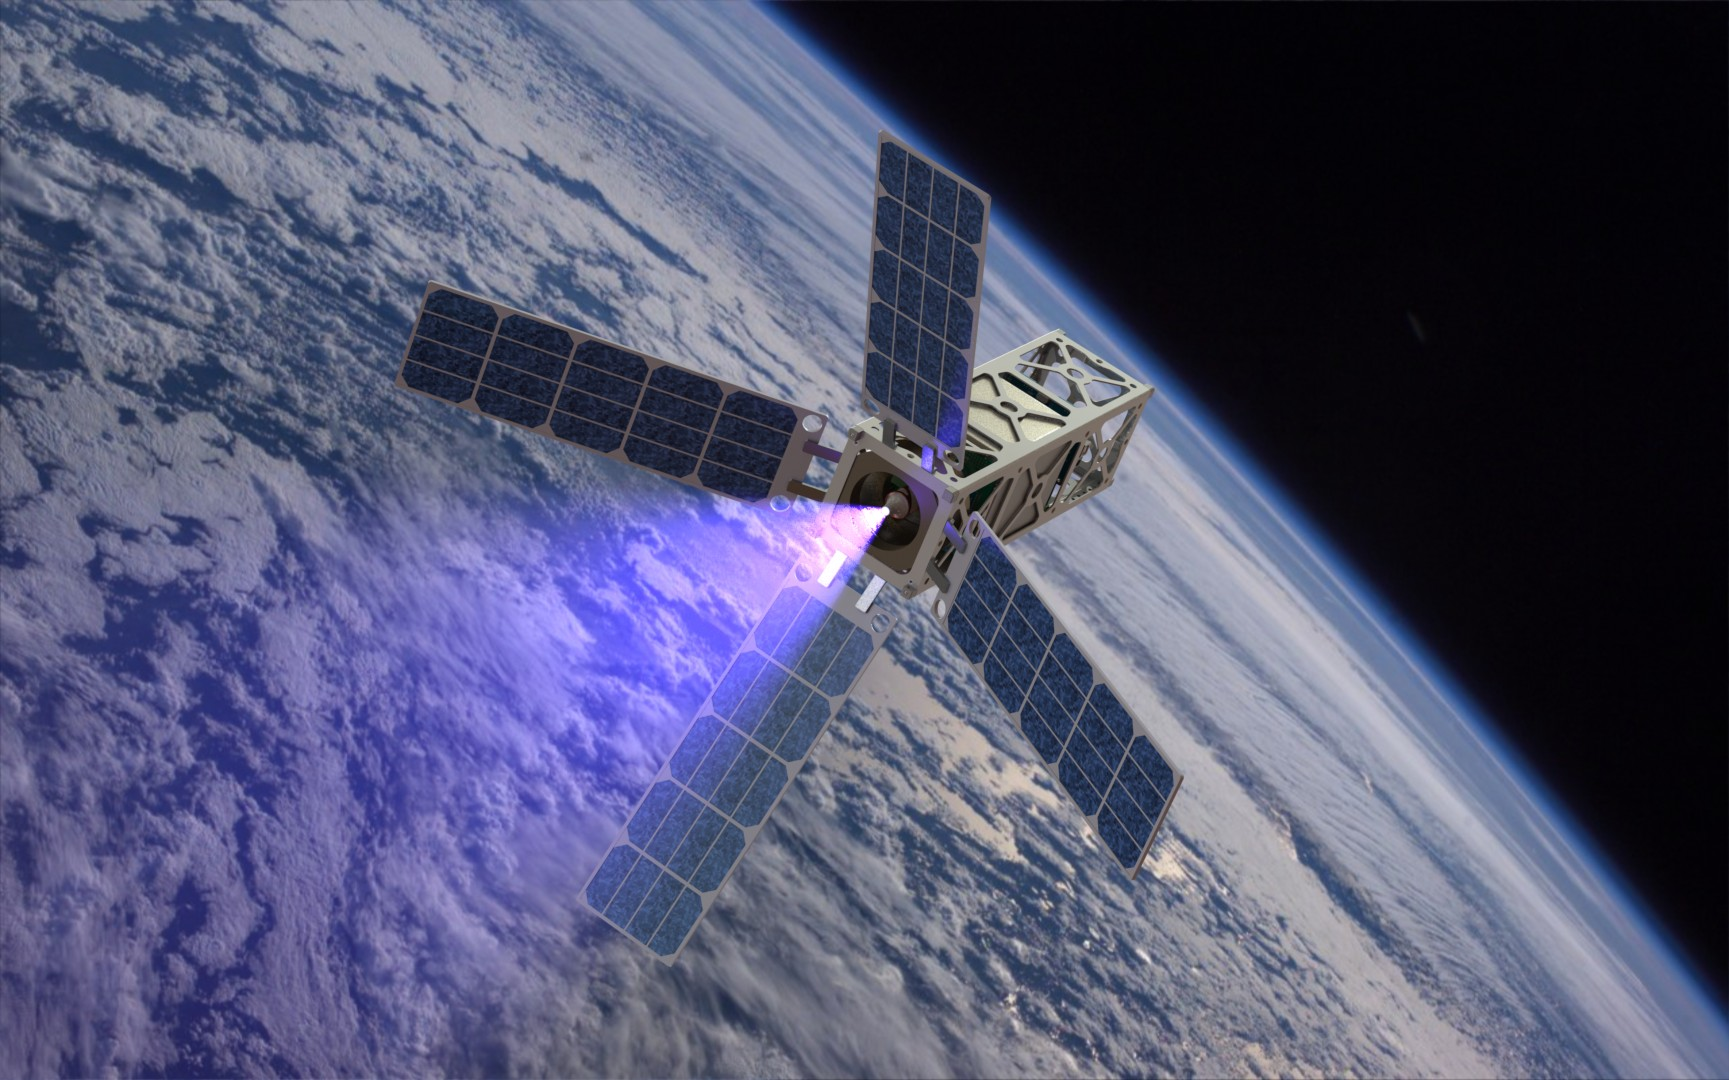
\includegraphics[height=0.5\textheight]{figures/patriot_plume.jpg}
    ~
    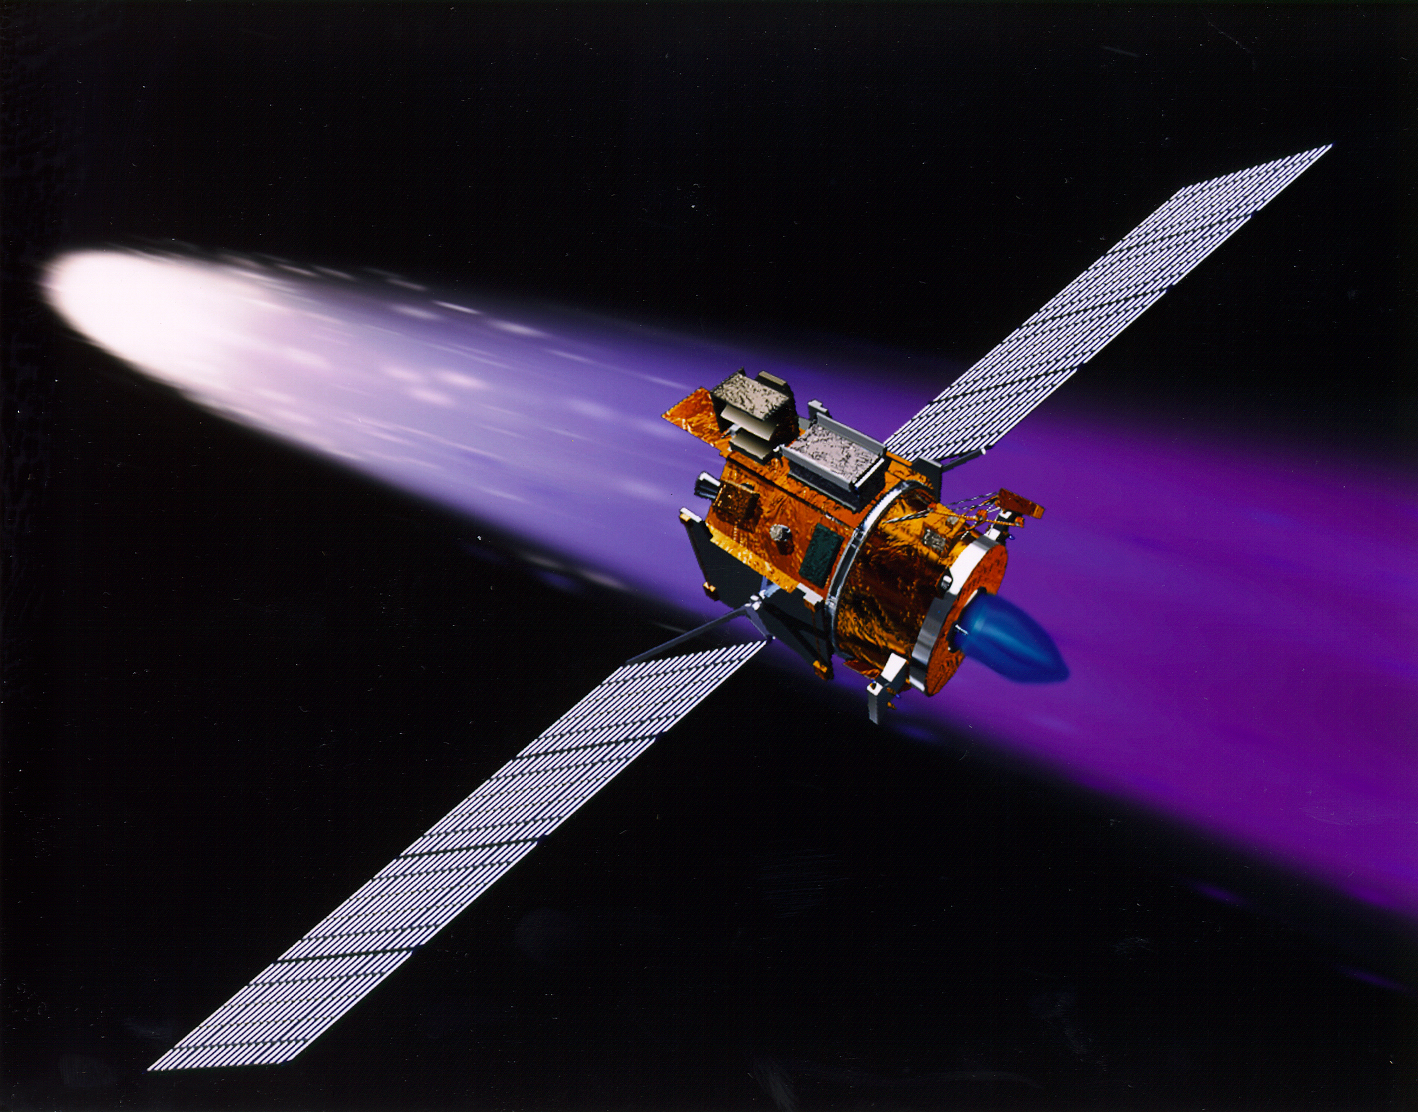
\includegraphics[height=0.5\textheight]{figures/deepspace1.jpg}
\end{center}
\end{frame}   %-----------------------------%

\begin{frame}{Asteroids}
\begin{itemize}
    \item Science - insight into the early formation of the solar system
    \item Mining - vast quantities of useful materials
    \item Impact - high risk from hazardous near-Earth asteroids
\end{itemize}    

\begin{center}
    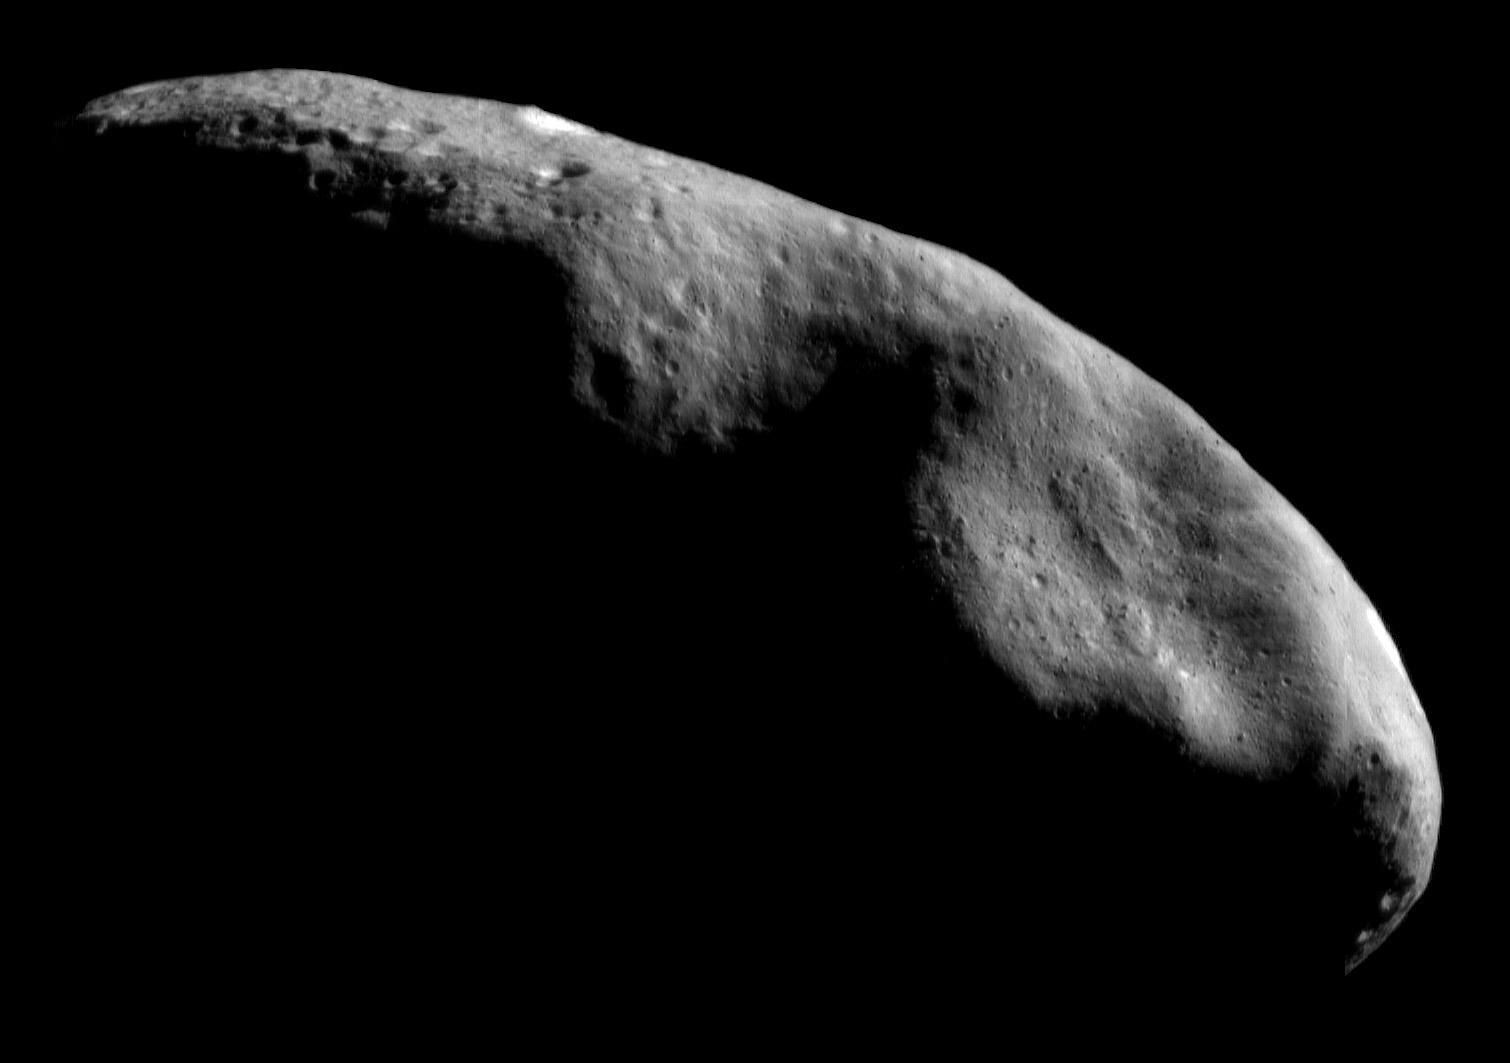
\includegraphics[height=0.5\textheight]{figures/2016AAS/near_mos_20001203_full.jpg}
    ~
    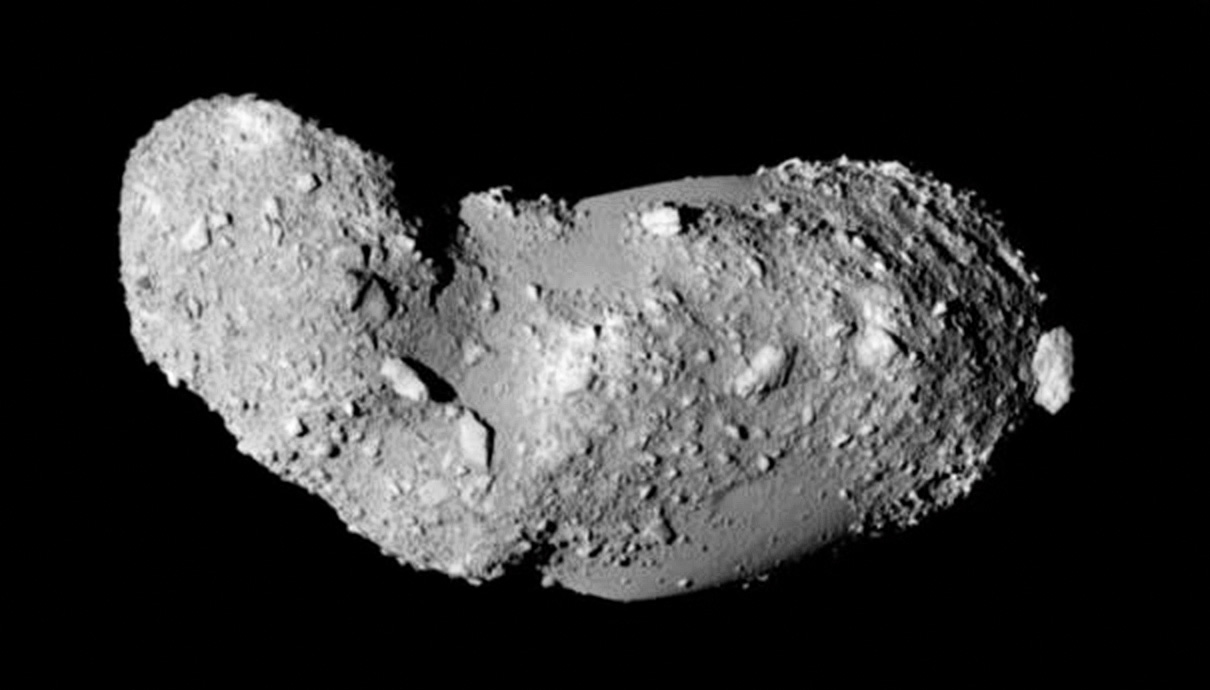
\includegraphics[height=0.5\textheight]{figures/2016AAS/Itokawa8_hayabusa_1210.jpg}
\end{center}
\end{frame}

\begin{frame}{Asteroid Mining}
    \begin{itemize}
      \item Useful materials can be extracted from asteroids to support:
      \begin{itemize}
          \item Propulsion, construction, life support, agriculture, and precious/strategic metals
      \end{itemize}
      \item Commercialization of near-Earth asteroids is feasible
    \end{itemize}

\pause

\begin{center}
\small
    \begin{tabular}{|l|r|r|}
        \hline 
        Element & Price (\SI{}{\$\per\kilo\gram}) & Sales (\SI{}{\$M\per\year}) \\
        \hline \hline 
        Phosphorous (P) & \num{0.08}  & \num{2167} \\
        Gallium (Ga) & \num{300.00}  & \num{1544} \\
        Germanium (Ge) & \num{745.00} & \num{6145} \\
        \hline \hline 
        Platinum (Pt) & \num{12394.00} & \num{1705} \\
        Gold (Au) & \num{12346.00} & \num{49} \\
        Osmium (Os) & \num{12860.00} & \num{307} \\
        \hline
    \end{tabular}
\end{center}

\end{frame}

\begin{frame}{Challenges} %-----------------------------%

\begin{itemize}
    \item Optimal Trajectory Design
        \begin{itemize}
            \item Orbital dynamics are nonlinear and chaotic
            \item Very sensitive to initial conditions
            \item Intuition required by designer to enable convergence
        \end{itemize}
    \pause
    \item Transfers using low-thrust propulsion
        \begin{itemize}
            \item Requires long periods of thrusting/coasting
            \item Small perturbations require accurate numerical integration
            \item Difficult to capture the long-term effects accurately
        \end{itemize}
    \pause
    \item Direct Optimal Control
        \begin{itemize}
            \item Reformulate problem as parameter optimization
            \item Allows for use of nonlinear programming methods
            \item High dimensional problem and computationally intensive
            \item Results in suboptimal solutions due to discretization
        \end{itemize}
\end{itemize}
\end{frame}   %-----------------------------%

\subsection{Approach}

\begin{frame}{Proposed Approach} % -----------------------------------%
  \begin{itemize}
      \item \Emph{Reachability set} on \Poincare section allows for systematic transfer design
        \begin{itemize}
            \item Transfer design on lower dimensional subspace
            \item Simple method to incorporate effects of low-thrust 
            \item Avoids the issue of determining initial conditions
        \end{itemize}
        \pause
      \item Extension of previous work in planar three-body problem     
  \end{itemize}

  \note[itemize]{
    \item Reachability set avoids the need to pick initial conditions
    \item We compute on a lower dimensional surface
  }
\end{frame} %--------------------------------------%

\begin{frame}{\Poincare map}
\begin{itemize}
    \item Intersection of a periodic orbit with a lower dimensional subspace, called the \Poincare section
    \pause
        \begin{itemize}
            \item Can be considered a discrete map 
        \end{itemize}
        \pause
    \item Useful for investigating the stability and structure 
    \pause
    \item Define a \Poincare section \( \Sigma \) 
        \begin{itemize}
            \item Used for initial and target periodic orbits
            \item Subspace for the \Emph{reachability set}
        \end{itemize}
\end{itemize}

\begin{align*}
    \Sigma = \braces{\parenth{x, \dot{x}, z, \dot{z}} | y(t_f) = 0 }
\end{align*}

\end{frame}

\begin{frame}{Reachability Set}

\begin{itemize}
    \item Set of states achievable from a given initial condition over fixed \( t_f \) s.t. maximum control constraint
    \begin{align*}
        R( \vecbf{x}_0, \mathcal{U} , t_f) = \braces{ \vecbf{x}_f \subseteq \mathcal{X} | \exists \vecbf{u} \in \mathcal{U}, \vecbf{x}(t_f) = \vecbf{x}_f }
    \end{align*}
    \pause
    \item Directly derivable from optimal control
    \item Frequently used for safety planning, e.g. air traffic collision avoidance
    \pause
    \item We extend its use to the design of spacecraft transfers
\end{itemize}

\end{frame}

\begin{frame}{Reachability Set on \Poincare section} % -----------------------------------%

\begin{itemize}
    \item Generate the reachability set on a \Poincare section
    \[
        \Sigma = \braces{\parenth{x, \dot{x}, z, \dot{z}} | y(t_f) = 0 }
    \]
    \item Control input is chosen to enlarge the reachable set
\end{itemize}
\pause
\begin{figure}
    \centering
    \begin{scaletikzpicturetowidth}{0.4\textwidth}
    \begin{tikzpicture}[scale=\tikzscale]
        \coordinate [label=left:\textcolor{black}{\large \(\vecbf{x}_0\)}] (x0) at (-1,-2);
        \coordinate [label=below:\textcolor{black}{\large  \(\vecbf{x}_n\)}] (xn) at (1,1);
        \coordinate [label=left:\textcolor{black}{\large  \(\Sigma\)}] (sigma) at (-4,3);
        %\coordinate [label=below:\textcolor{black}{\large  \(P(\vec{x})\)}] (P) at (0,-3.5);
        % define the path of the flow with coordinates
        \coordinate [label=right:\textcolor{black}{}] (f1) at (5,-2);
        \coordinate [label=below:\textcolor{black}{\large  \(\psi(t,\vecbf{x}_0)\)}] (f2) at (2,-5);
        \coordinate [label=right:\textcolor{black}{}] (f3) at (-4,-4);
        \coordinate [label=right:\textcolor{black}{}] (f4) at (-4,-1);
        
    %   \draw[help lines] (-10,-10) grid (10,10); %grid
        \filldraw [black] (x0) circle [radius=3pt];
        \filldraw [black] (xn) circle [radius=3pt];
    
        \draw [ultra thick,black,->-](x0) to[out=20,in=90,distance=2cm] (f1) to[out=-90,in=0,distance=2cm] (f2) to[out=180,in=-45,distance=2cm] (f3) to[out=135,in=-135,distance=2cm] (f4) ;
        \draw [ultra thick, black,dashed,->] (f4) to[out=45,in=180,distance=1cm] ($(xn)-(2,0)$);
        
        \draw [ultra thick] plot [smooth cycle, tension=0.1, rotate=5] coordinates { (-4,-3) (4,-3) (4,3) (-4,3) };
    
        \draw [thick,dashed] (xn) circle [radius=2cm]; % reachability set
    
        \draw [thick,->] (xn) -- ($(xn) + (2.5,0)$);
        \draw [thick,rotate=45,->] (xn) -- ($(xn) + (2.5,0)$);
        \draw ($(xn) + (1,0)$) arc [start angle=0,end angle=45, radius=1];
        \node [draw=none] at (2.8,1.5) {\large \(\phi_d\)};
        \draw [decorate,decoration={brace,amplitude=5pt},rotate=45] (xn) -- ($(xn) + (2,0)$);
        \node [draw=none] at ($ (xn) + (0,1) $) {\large \( J \)};
    \end{tikzpicture}
    \end{scaletikzpicturetowidth}
\end{figure}

\end{frame} %--------------------------------------%

\begin{frame}{Optimal Control Problem}
\begin{itemize}
    \item Reachability defined as distance between controlled and uncontrolled states
    {\small
        \[
            J = -\frac{1}{2} \left( \vecbf{x}(t_f) - \vecbf{x}_{n}(t_f)\right)^T 
            Q
            \left( \vecbf{x}(t_f) - \vecbf{x}_{n}(t_f)\right) 
        \]
    }
    \pause
    \item Terminal constraints used to ensure correct section and specific direction on \( \Sigma \in \R^4 \)
    {\small
        \begin{align*}\label{eq:terminal_constraints}
            \begin{split}
                m_1 &= y = 0  \\
                m_2 &= \parenth{\sin \phi_{1_{d}}} \parenth{ x_1^2 + x_2^2 + x_3^2 + x_4^2} - x_1^2 = 0 \\
                m_3 &= \parenth{\sin \phi_{2_{d}}} \parenth{ x_2^2 + x_3^2 + x_4^2} - x_2^2 = 0\\
                m_4 &= \parenth{\sin \phi_{3_{d}}} \parenth{ 2 x_3^2 + 2 x_3 \sqrt{x_4^2 + 2 x_4^2}} - x_3 - \sqrt{x_4^2 + x_3^2} = 0 
            \end{split}
        \end{align*}
    }
    \pause
    \item Control constraint used to emulate realistic system
        {\small
        \[
            c(\vecbf{u}) = \vecbf{u}^T \vecbf{u} - u_m^2 \leq 0 
        \]
        }
\end{itemize}

\end{frame}

\begin{frame}{Two Point Boundary Value Problem}
\begin{itemize}
    \item Multiple shooting used to solve necessary conditions
    \pause
    \item Approximate the reachable set via \( \phi_1, \phi_2, \phi_3 \) 
    \pause
    \item From the reachable set we chose the state which minimizes \( d \) 
    \item Compute another reachable set if target is not feasible
\end{itemize}

\begin{align*}
    d = \sqrt{k_x \parenth{x_f - x_t }^2 + k_z \parenth{z_f - z_t }^2 + k_{\dot{x}}\parenth{\dot{x}_f - \dot{x}_t }^2 + k_{\dot{z}}\parenth{\dot{z}_f - \dot{z}_t }^2} 
\end{align*}

\end{frame}

\begin{frame}{Numerical Simulation}
\begin{itemize}
    \item Reachability approach applied to two dynamical systems
    \begin{itemize}
        \item Planar Circular Restricted Three Body Problem
        \item Two-body motion about asteroids
    \end{itemize}
    \item Extension from planar to 3D motion 
    \item Inclusion of complex gravitional field
\end{itemize}

\end{frame}

\subsection{CRTBP}

\begin{frame}{Geostationary to \( L_1 \) transfer} %----------------------------------------------------%
\begin{itemize}
       \item Tranfer for geostationary orbit to a periodic orbit about \( L_1\)
       \item Multiple iterations of reachable set
\end{itemize}

\begin{figure}
       \centering
       \begin{subfigure}[htbp]{0.5\textwidth}
               \only<1>{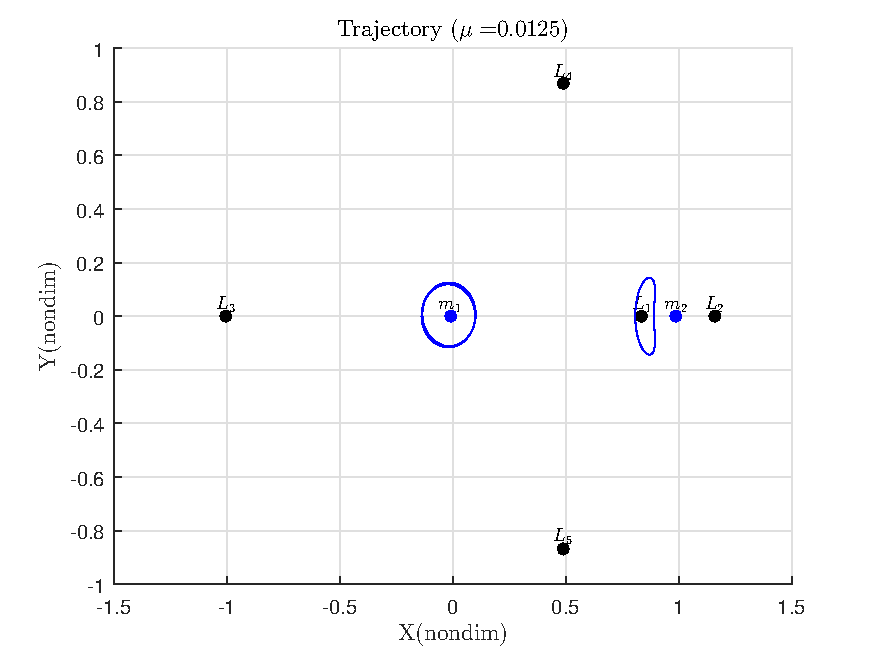
\includegraphics[width=\textwidth]{initial_final}  }
               \only<2>{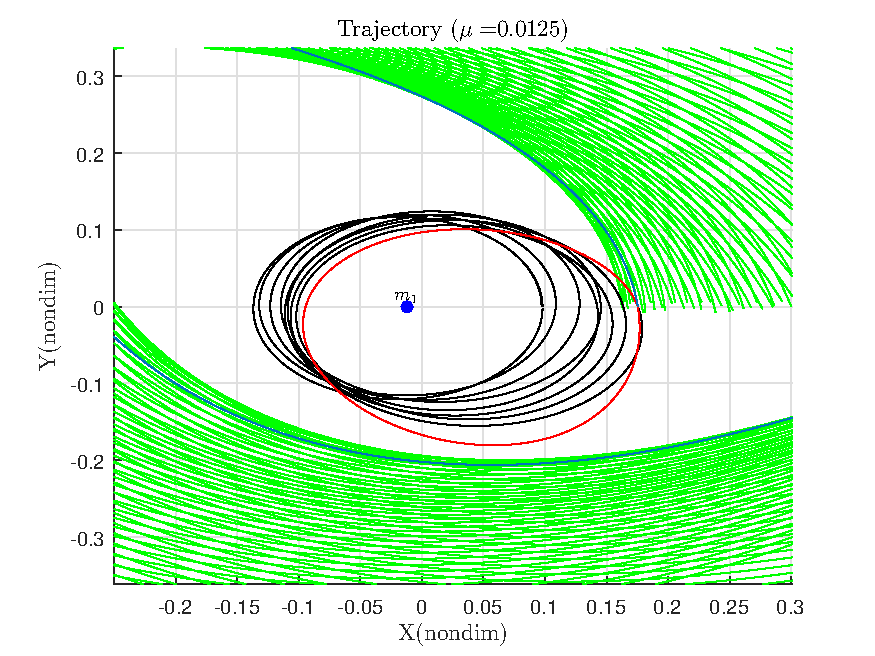
\includegraphics[width=\textwidth]{geo_transfer_zoom}  }
       \end{subfigure}~
       \begin{subfigure}[htbp]{0.5\textwidth}
               \only<1>{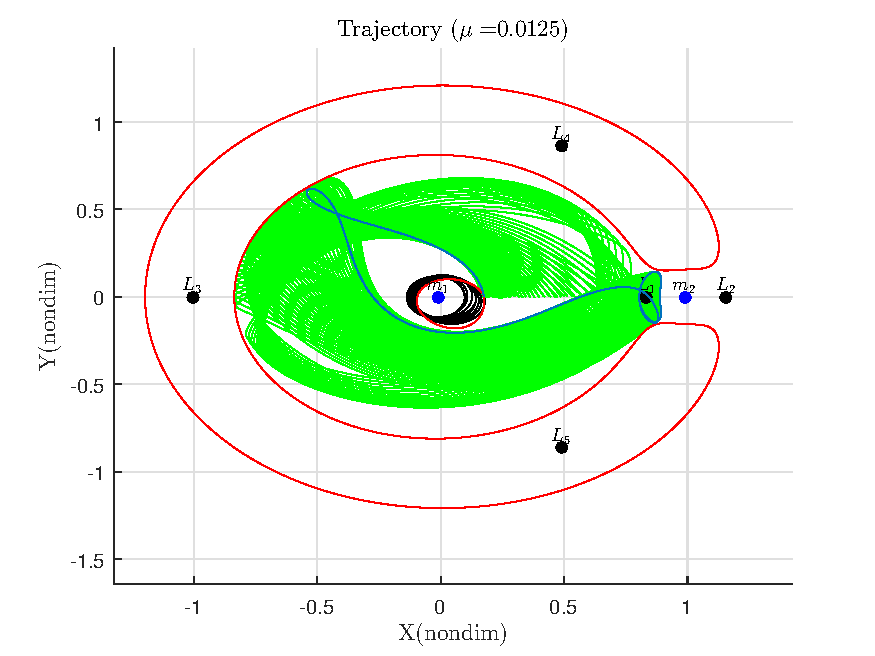
\includegraphics[width=\textwidth]{geo_transfer_full} }
               \only<2>{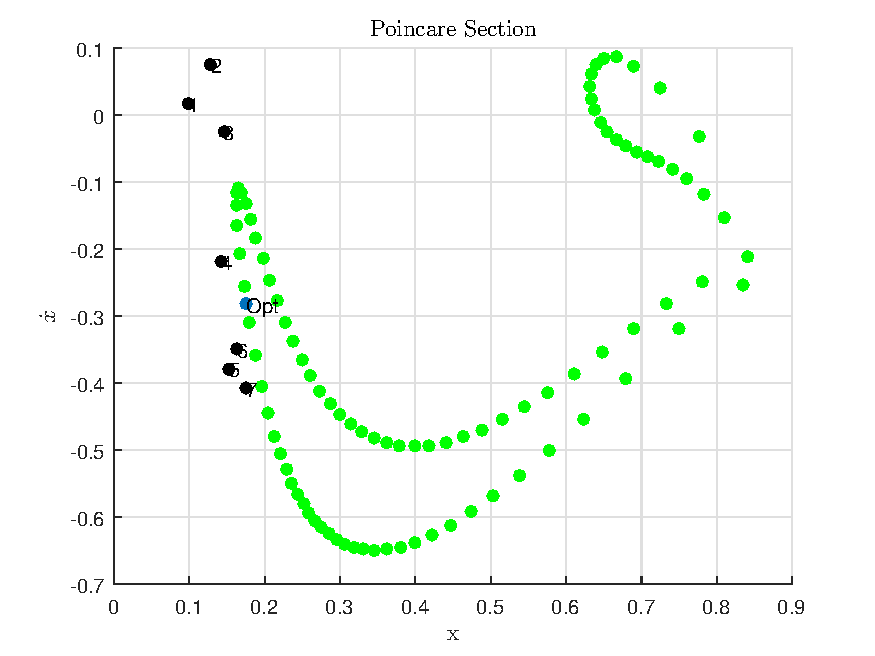
\includegraphics[width=\textwidth]{poincare}}
       \end{subfigure}
       \end{figure}

\end{frame} %--------------------------------------------%

\subsection{4769 Castalia}

\begin{frame}{Polyhedron Gravitation Model}

\begin{itemize}
    \item Potential is a function of only the shape model
    \item Globally valid, closed-form expression of potential
    \item Exact potential assumes a constant density 
    \item Accuracy solely dependent on shape model
\end{itemize}
\only<2>{
\begin{align*}\label{eq:potential}
    U(\vecbf{r}) &= \frac{1}{2} G \sigma \sum_{e \in \text{edges}} \vecbf{r}_e \cdot \vecbf{E}_e \cdot \vecbf{r}_e \cdot L_e - \frac{1}{2}G \sigma \sum_{f \in \text{faces}} \vecbf{r}_f \cdot \vecbf{F}_f \cdot \vecbf{r}_f \cdot \omega_f 
\end{align*}
}
\only<3>{
\begin{center}
  \animategraphics[autoplay,loop,height=0.6\textheight]{30}{./animation/2016AAS/castalia/IMG}{00001}{00999}~\hfill
  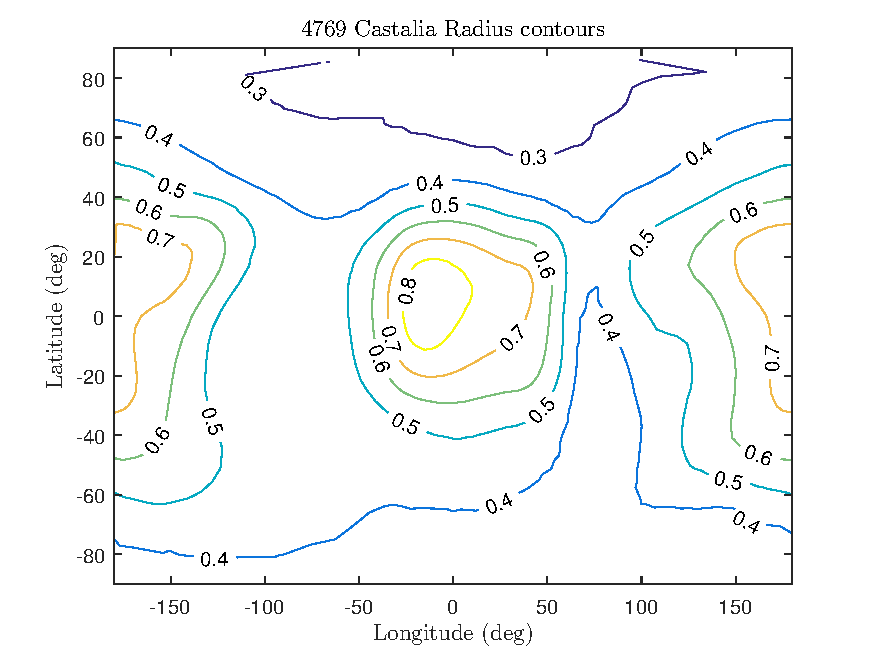
\includegraphics[width=0.6\textheight]{figures/2016AAS/radius_contour.pdf}
\end{center}
}

\end{frame}

\begin{frame}{4769 Simulation}

\begin{itemize}
    \item Generate the reachability set through discretization of \( \phi_i \)
    \item Visualize \( \Sigma \in \R^4 \) through the use of two 2-D sections
    \pause
    \item Control input allows for large deviation in velocity components
\end{itemize}

\begin{center}
    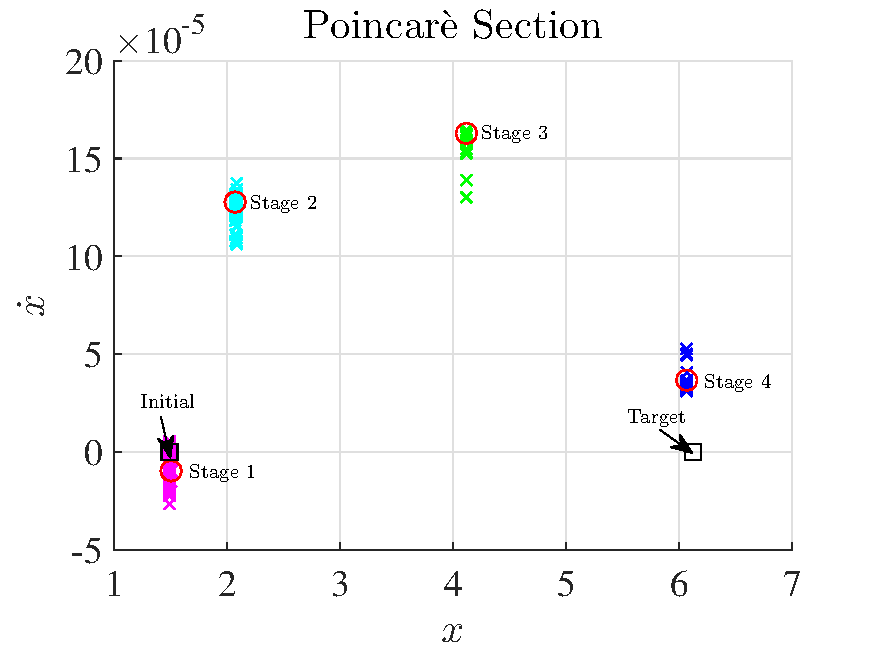
\includegraphics[width=0.5\textwidth]{figures/2016AAS/poincare_xvsxdot.pdf}
    \hfill
    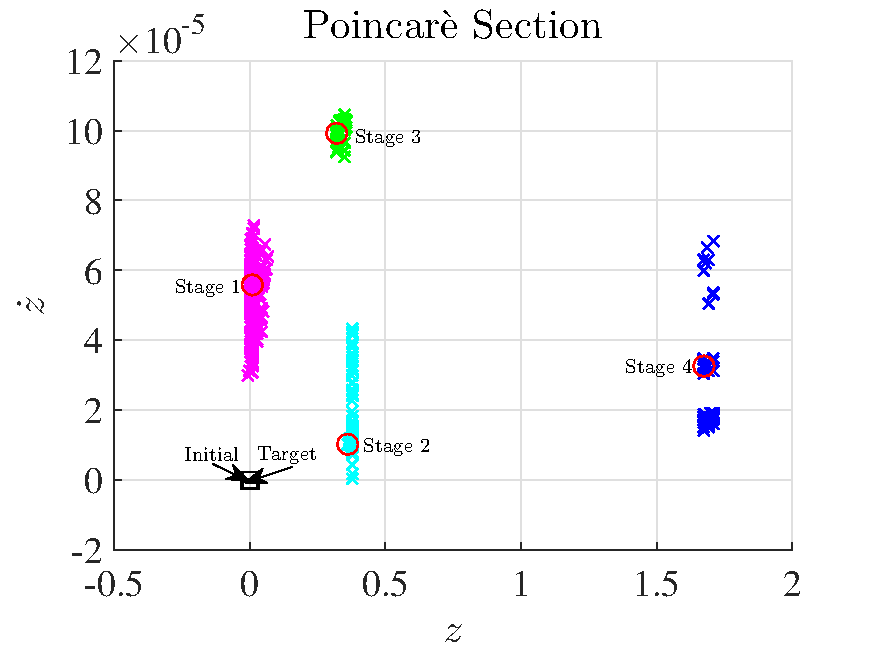
\includegraphics[width=0.5\textwidth]{figures/2016AAS/poincare_zvszdot.pdf}
\end{center}

\end{frame}

\begin{frame}{Simulation}
    \begin{itemize}
        \item Four iterations of the reachable state to meet the target set
        \item Final transfer is computed with a fixed terminal state constraint
    \end{itemize}

    \begin{center}
        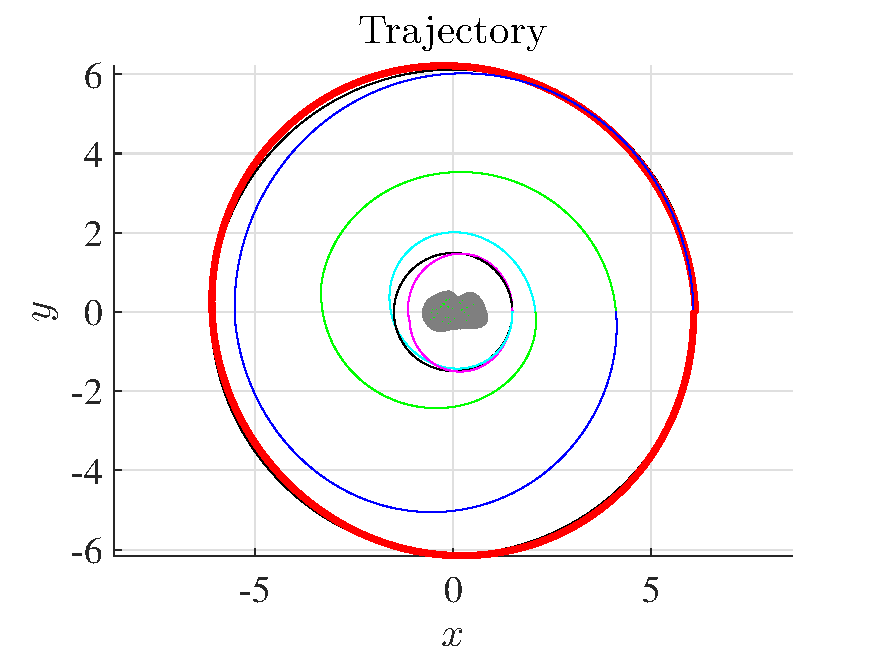
\includegraphics[width=0.5\textwidth]{figures/2016AAS/trajectory.pdf}
        \hfill
        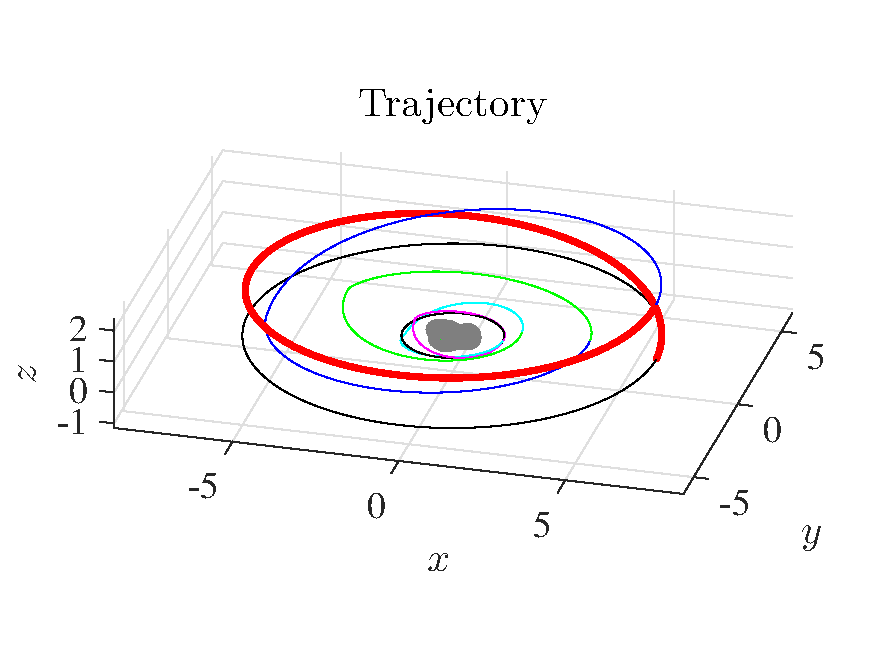
\includegraphics[width=0.5\textwidth]{figures/2016AAS/trajectory_3d.pdf}
    \end{center}

\end{frame}

\begin{frame}{Complete transfer}
\begin{itemize}
    \item We can visualize the complete trajectory in both the body and inertial frames
\end{itemize}

\begin{center}
  \animategraphics[autoplay,loop,width=0.5\textwidth]{30}{./animation/2016AAS/body/IMG}{00001}{01499}~\hfill
  \animategraphics[autoplay,loop,width=0.5\textwidth]{30}{./animation/2016AAS/inertial/IMG}{00001}{01499}
\end{center}

\end{frame}